\documentclass[hidelinks,12pt]{article}
\usepackage[left=0.25cm,top=1cm,right=0.25cm,bottom=1cm]{geometry}
%\usepackage[landscape]{geometry}
\textwidth = 20cm
\hoffset = -1cm
\usepackage[utf8]{inputenc}
\usepackage[spanish,es-tabla]{babel}
\usepackage[autostyle,spanish=mexican]{csquotes}
\usepackage[tbtags]{amsmath}
\usepackage{nccmath}
\usepackage{amsthm}
\usepackage{amssymb}
\usepackage{mathrsfs}
\usepackage{graphicx}
\usepackage{subfig}
\usepackage{standalone}
\usepackage[outdir=./Imagenes/]{epstopdf}
\usepackage{siunitx}
\usepackage{physics}
\usepackage{color}
\usepackage{float}
\usepackage{hyperref}
\usepackage{multicol}
%\usepackage{milista}
\usepackage{anyfontsize}
\usepackage{anysize}
%\usepackage{enumerate}
\usepackage[shortlabels]{enumitem}
\usepackage{capt-of}
\usepackage{bm}
\usepackage{relsize}
\usepackage{placeins}
\usepackage{empheq}
\usepackage{cancel}
\usepackage{wrapfig}
\usepackage[flushleft]{threeparttable}
\usepackage{makecell}
\usepackage{fancyhdr}
\usepackage{tikz}
\usepackage{bigints}
\usepackage{scalerel}
\usepackage{pgfplots}
\usepackage{pdflscape}
\pgfplotsset{compat=1.16}
\spanishdecimal{.}
\renewcommand{\baselinestretch}{1.5} 
\renewcommand\labelenumii{\theenumi.{\arabic{enumii}})}
\newcommand{\ptilde}[1]{\ensuremath{{#1}^{\prime}}}
\newcommand{\stilde}[1]{\ensuremath{{#1}^{\prime \prime}}}
\newcommand{\ttilde}[1]{\ensuremath{{#1}^{\prime \prime \prime}}}
\newcommand{\ntilde}[2]{\ensuremath{{#1}^{(#2)}}}

\newtheorem{defi}{{\it Definición}}[section]
\newtheorem{teo}{{\it Teorema}}[section]
\newtheorem{ejemplo}{{\it Ejemplo}}[section]
\newtheorem{propiedad}{{\it Propiedad}}[section]
\newtheorem{lema}{{\it Lema}}[section]
\newtheorem{cor}{Corolario}
\newtheorem{ejer}{Ejercicio}[section]

\newlist{milista}{enumerate}{2}
\setlist[milista,1]{label=\arabic*)}
\setlist[milista,2]{label=\arabic{milistai}.\arabic*)}
\newlength{\depthofsumsign}
\setlength{\depthofsumsign}{\depthof{$\sum$}}
\newcommand{\nsum}[1][1.4]{% only for \displaystyle
    \mathop{%
        \raisebox
            {-#1\depthofsumsign+1\depthofsumsign}
            {\scalebox
                {#1}
                {$\displaystyle\sum$}%
            }
    }
}
\def\scaleint#1{\vcenter{\hbox{\scaleto[3ex]{\displaystyle\int}{#1}}}}
\def\bs{\mkern-12mu}


\usepackage{apacite}
\title{Funciones Gamma y Beta \\[0.3em]  \large{Matemáticas Avanzadas de la Física}\vspace{-3ex}}
\author{M. en C. Gustavo Contreras Mayén}
\date{ }
\begin{document}
\vspace{-4cm}
\maketitle
\fontsize{14}{14}\selectfont
\tableofcontents
\newpage

\section{Introducción.}

\subsection{Integrales como funciones.}

Las integrales son uno de los medios matemáticos más convenientes con los que se pueden definir nuevas funciones.
\par
Si el integrando o los límites de integración incluyen parámetros, esos parámetros pueden tratarse como variables y la integral misma como una función de esos parámetros.
\par
Haremos una revisión de algunas funciones más importantes que normalmente se definen en términos de integrales.

\subsection{Funciones de apoyo.}

La función Gamma $\Gamma$ aparece ocasionalmente en problemas de física tales como:
\begin{enumerate}
\item Cálculo de probabilidades en mecánica estadística.
\item La normalización de las funciones de onda para el potencial de Coulomb en mecánica cuántica.
\end{enumerate}
En realidad la función $\Gamma$ tiene pocas aplicaciones directas en física, sin embargo es importante porque nos permite desarrollar otras funciones que si tienen una aplicación directa en la física, como por ejemplo: las funciones de Bessel.
\par
La relación entre las funciones $\Gamma$ y $B$ también nos permitirán expresar de manera más compacta los resultados que se obtendrán al resolver ciertas ecuaciones diferenciales que veremos a lo largo del curso.
\par
Es por ello que al manejar debidamente estas funciones (y sus variantes), tendremos más herramientas para nuestro objetivo: resolver un problema de la física mediante el uso de funciones especiales, y con ello, interpretar el fenómeno que estudiamos.
\par
\textbf{Nota importante: }Para el manejo de estas funciones será necesario un trabajo fluido en cuanto a la solución de integrales tanto definidas como indefinidas, por lo que tendrás oportunidad de ejercitar lo aprendido en los cursos de cálculo.
\par
Es cierto que existe software matemático (Wolfram, Mathematica, etc.) que te devolverá la solución para algunas integrales, pero confiamos en que utilizarás esas herramientas para corroborar tus resultados, es decir, esperamos que resuelvas \enquote{a mano} cada una de las integrales que se te presenten.
\par
Recuerda que es necesario contar con la evidencia de tu trabajo en la solución de un ejercicio, así que como diría un maestro: \enquote{hay que arrastrar el lápiz}.

% Referencia: Boas (2005) Chap. 11 Special Functions
\section{La función factorial.}

\subsection{Definición.}

Calculemos el valor de la siguiente integral, para $\alpha > 0$:
\begin{align}
\int_{0}^{\infty} e^{-\alpha \, x} \dd{x} = - \dfrac{1}{\alpha} e^{-\alpha \, x}\eval_{0}^{\infty} = \dfrac{1}{\alpha}
\label{eq:ecuacion_02_01}
\end{align}
Con el fin de mantener una buena legibilidad, escribiremos el argumento de la función exponencial como superíndice $e^{-\alpha \, x}$, pero si el argumento es extenso, la función se escribirá como $\exp(-\alpha \, x)$.
\par
Diferenciamos con respecto a $\alpha$ ambos lados de la ec. (\ref{eq:ecuacion_02_01}):
\begin{align*}
\int_{0}^{\infty} - x \, e^{-\alpha \, x} \dd{x} = - \dfrac{1}{\alpha^{2}} &= \int_{0}^{\infty} x \, e^{-\alpha \, x} \dd{x} = \dfrac{1}{\alpha^{2}} \\[0.5em]
&= \int_{0}^{\infty} x^{2} \, e^{-\alpha \, x} \dd{x} = \dfrac{2}{\alpha^{3}} \\[0.5em]
&= \int_{0}^{\infty} x^{3} \, e^{-\alpha \, x} \dd{x} = \dfrac{3!}{\alpha^{4}} \\
& \vdots
\end{align*}
La expresión general luego de $n$ pasos de diferenciación con respecto a $\alpha$ es:
\begin{align}
\int_{0}^{\infty} x^{n} \, e^{-\alpha \, x} \dd{x} = \dfrac{n!}{\alpha^{n+1}}
\label{eq:ecuacion_02_02}
\end{align}
Haciendo que $\alpha = 1$, se obtiene
\begin{align}
\int_{0}^{\infty} x^{n} \, e^{-x} \dd{x} = n! \hspace{1cm} n = 1, 2, 3, \ldots
\label{eq:ecuacion_02_03}
\end{align}
Así tenemos una integral definida cuyo valor es $n!$ para un entero positivo $n$.
\par
Usando la ec. (\ref{eq:ecuacion_02_03}) le podemos dar un significado al valor de $0!$: si hacemos $n = 0$, ocurre:
\begin{align}
0! = \int_{0}^{\infty} e^{-x} \dd{x} = -e^{x}\eval_{0}^{\infty} = 1
\label{eq:ecuacion_02_04}
\end{align}

\section{Doble factorial.}

\subsection{Notación.}

En varios problemas de la física, en particular con los \emph{polinomios de Legendre}, encontraremos productos de enteros impares positivos y de pares positivos, por conveniencia, definimos el doble factorial:
\begin{align}
\begin{aligned}
1 \cdot 3 \cdot 5 \cdots (2 \, n+1) &= (2 \, n+1) !! \\
2 \cdot 4 \cdot 6 \cdots (2 \, n) &= (2 \, n) !!
\end{aligned}
\label{eq:ecuacion_10_33b}
\end{align}
Que están relacionados con la función factorial
\begin{align}
\begin{aligned}
(2 \, n)!! &=  2^{n} \: n! \\[1em]
(2 \, n+1)!! &= \dfrac{(2 \, n+1)!}{2^{n} \, n!}
\end{aligned}
\label{eq:ecuacion_10_33c}
\end{align}
También se define $(-1)!! = 1$, un caso especial que no se obtiene de la ec. (\ref{eq:ecuacion_10_33c})

\section{Función Gamma.}

\subsection{Definición.}

En el desarrollo que hemos hecho, $n$ es un número entero no negativo, es natural definir la función factorial para un $n$ no entero mediante la integral de la ec.(\ref{eq:ecuacion_02_03}).
\par
No hay ninguna objeción en la notación $n!$ para $n$ no entero, pero es habitual reservar la notación factorial para $n$ entero.
\par
Para el caso de una función para evaluar el factorial de un $n$ no entero, entonces llamaremos a esa función: la función gamma $(\Gamma)$.
\par
También es una práctica bastante común reemplazar $n$ por la letra $p$ cuando queremos decir que no es necesariamente un número entero.
\par
Siguiendo estas convenciones, se define la función Gamma para cualquier $p > 0$:
\begin{align}\addtolength{\fboxsep}{5pt}\boxed{
\Gamma (p) = \int_{0}^{\infty} x^{p-1} \, e^{-x} \dd{x}, \hspace{1cm} p > 0}
\label{eq:ecuacion_03_01}
\end{align}
\begin{enumerate}
\item Para $0 < p < 1$ la integral (\ref{eq:ecuacion_03_01}) se hace impropia, ya que el término $x^{p-1}$ tiende a infinito en el límite inferior.
\item Para $p > 0$ se tiene una integral que converge.
\item Para $p \leq 0$ la integral diverge y no se puede usar para definir $\Gamma (p)$, más adelante veremos cómo definir  $\Gamma (p)$ para $p \leq 0$.
\end{enumerate}

\subsection{Primeras propiedades.}

De las ecs. (\ref{eq:ecuacion_03_01}) y (\ref{eq:ecuacion_02_03}), se tiene que:
\begin{align}
\begin{aligned}
\Gamma (n) &= \int_{0}^{\infty} x^{n-1} \, e^{-x} \dd{x} = (n -1)! \\[1em]
\Gamma (n+1) &= \int_{0}^{\infty} x^{n} \, e^{-x} \dd{x} = n!
\end{aligned}
\label{eq:ecuacion_03_02}
\end{align}
Entonces:
\begin{align*}
\Gamma (1) &= 0! = 1 \\
\Gamma (2) &= 1! = 1 \\
\Gamma (3) &= 2! = 2 \\
\Gamma (4) &= 3! = 6 \\
&\ldots \\
\Gamma (n) &= n-1!
\end{align*}
Donde el factorial de un entero positivo $n$, es el que conocemos del álgebra.
\par
Al reemplazar $p$ por $p+1$ en la ec. (\ref{eq:ecuacion_03_01}) nos deja:
\begin{align}
\Gamma (p+1) = \int_{0}^{\infty} x^{p} \, e^{-x} \dd{x} = p!, \hspace{1cm} p > -1
\label{eq:ecuacion_03_03}
\end{align}
En algunos textos se ocupa la notaciona factorial $p! = \Gamma (p+1)$, aunque $p$ es un no entero.

\subsection{Relación de recurrencia.}

Al integrar por partes la ec. (\ref{eq:ecuacion_03_03}), haciendo
\begin{align*}
x^{p} =  u \hspace{2cm} e^{-x} \dd{x} =  \dd{v}
\end{align*}
Entonces tenemos que
\begin{align*}
\dd{u} &= p \, x^{p-1} \dd{x}, \hspace{1cm} v = - e^{-x} \\[1em]
\Gamma (p+1) &= -x^{p} \, e^{-x} \displaystyle \eval_{0}^{\infty} - \displaystyle \int_{0}^{\infty} \left(-e^{-x} \right) \, p \, x^{p-1} \dd{x} = \\[1em]
&= p \displaystyle \int_{0}^{\infty} x^{p-1} \, e^{-x} \dd{x}
\end{align*}
Donde reconocemos la integral que define a la función Gamma, entonces obtenemos la regla de recurrencia:  
\begin{align}\addtolength{\fboxsep}{5pt}\boxed{
\Gamma (p+1) = p \, \Gamma (p)}
\label{eq:ecuacion_03_04}
\end{align}
Que es de utilidad para simplificar expresiones que involucran a la función $\Gamma$.

\subsection{Función Gamma para \texorpdfstring{$p < 0$}{p < 0}.}

Para valores $p < 0$, la función $\Gamma (p)$ no se ha definido hasta el momento.
\par
Ocuparemos la relación de recursividad ec. (\ref{eq:ecuacion_03_04}) para resolverla. Entonces:
\begin{align}\addtolength{\fboxsep}{5pt}\boxed{
\Gamma (p) = \dfrac{1}{p} \, \Gamma (p + 1)}
\label{eq:ecuacion_04_01}
\end{align}
que define la función $\Gamma$ para valores $p < 0$
\par
Veamos un par de ejemplos: 
\begin{enumerate}
\item  Se quiere obtener el valor de $\Gamma (-0.3)$, entonces podemos resolverlo de la siguiente manera:
\begin{align*}
\Gamma (-0.3) = - \dfrac{1}{0.3} \, \Gamma (0.7)
\end{align*}
\item  Se quiere obtener el valor de $\Gamma (-0.3)$, entonces podemos resolverlo de la siguiente manera:
\begin{align*}
\Gamma (-1.3) = - \dfrac{1}{(-1.3)(-0.3)} \, \Gamma (0.7)
\end{align*}
\end{enumerate}
Los valores de la función $\Gamma$ se pueden obtener de tablas, pero lo más práctico es ocupar el software matemático (Wolfram, Mathematica) o lenguajes de programación que incluyen librerías científicas, como \texttt{python}.
\par
De este y el uso sucesivo de la ec. (\ref{eq:ecuacion_04_01}) se deduce que la función $\Gamma (p)$ tiende a infinito no solo en cero sino también en todos los enteros negativos.
\par
En los intervalos entre los enteros negativos, alterna valores positivos y negativos, negativo de 0 a -1, positivo de -1 a -2, y así sucesivamente, como puede ver en la siguiente figura (\ref{fig:figura_plot_gamma}).
\begin{figure}[H]
   \centering
   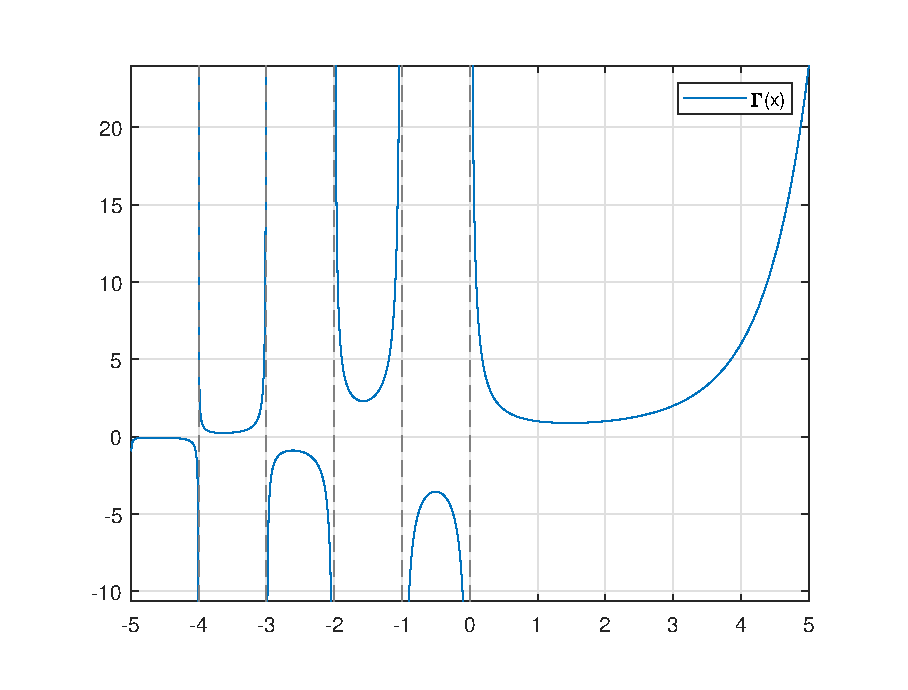
\includegraphics[scale=0.75]{Imagenes/Plot_Gamma.eps}
   \caption{Gráfica de la función Gamma $\Gamma (p)$}
   \label{fig:figura_plot_gamma}
\end{figure}

\section{Fórmulas que involucran a \texorpdfstring{$\Gamma (p)$}{G (p)}.}

\subsection{Algunas fórmulas.}

Como veremos a continuación, el desarrollo de las fórmulas para la función $\Gamma (p)$, se sigue de la definición, por lo que la operación algebraica y de solución de la integral es completamente posible.
\par
Nos interesa que dispongan de una relación de fórmulas y que puedan ocuparlas en donde sea necesario. Aunque las fórmulas son válidas, en el caso que se indique, deberán de demostrar la fórmula que vayan a utilizar.
\par 
Evaluemos $\Gamma (1/2)$. Usando la definición:
\begin{align}
\Gamma \left( \dfrac{1}{2}\right) = \int_{0}^{\infty} \dfrac{1}{\sqrt{t}} \, e^{-t} \dd{t}
\label{eq:ecuacion_05_01}
\end{align}
Toma en cuenta que no importa qué letra usemos para la variable \enquote{muda} de integración en una integral definida.
\par
Haciendo el cambio de variable en la ec. (\ref{eq:ecuacion_05_01}):
\begin{align*}
t = y^{2} \hspace{0.5cm} \Rightarrow \dd{t} = 2 \, y \dd{y}
\end{align*}
Entonces tenemos que
\begin{align*}
\Gamma \left( \dfrac{1}{2} \right) = \int_{0}^{\infty} \, e^{-y^{2}} \, 2 \, y \dd{y} = 2 \int_{0}^{\infty} \, e^{-y^{2}} \dd{y}
\end{align*}
Con $x$ como la variable \enquote{muda} de integración:
\begin{align}
\Gamma \left( \dfrac{1}{2} \right) = 2 \int_{0}^{\infty} \, e^{-x^{2}} \dd{x}
\label{eq:ecuacion_05_02}
\end{align}
Multiplicando las dos integrales de $\Gamma (1/2)$ para luego escribir el resultado como una integral doble:
\begin{align*}
\left[ \Gamma \left( \dfrac{1}{2} \right) \right]^{2} = 4 \int_{0}^{\infty} \, \int_{0}^{\infty} \, e^{-(x^{2} + y^{2})} \dd{x} \dd{y}
\end{align*}
Tenemos una doble integral sobre el primer cuadrante de una circunferencia, por lo que es más fácil evaluarla en coordenadas polares:
\begin{align*}
\left[ \Gamma \left( \dfrac{1}{2} \right) \right]^{2} &= 4 \int_{0}^{\pi/2} \, \int_{0}^{\infty} \, e^{-r^{2}} \, r \dd{r} \dd{\theta} = \\[0.5em]
&= 4 \, \dfrac{\pi}{2} \, \dfrac{e^{-r^{2}}}{-2}\eval_{0}^{\infty} = \\[0.5em]
&= \pi
\end{align*}
Entonces obtenemos la primera fórmula:
\begin{align}\addtolength{\fboxsep}{5pt}\boxed{
\Gamma \left( \dfrac{1}{2} \right) = \sqrt{\pi}}
\label{eq:ecuacion_05_03}
\end{align}

\subsection{Otras fórmulas.}

A continuación se enlistan algunas de las fórmulas que involucran a la función Gamma, toma en cuenta de que a pesar de que no se demuestra la expresión, en el caso de que la utilices para un ejercicio, deberás de presentar la respectiva demostración.
{%\fontsize{12}{12}\selectfont
\begin{align*}
\Gamma (x) &= (x - 1) \, \Gamma(x - 1) \hspace{1cm} x \neq 0, -1, -2, \ldots \\[0.75em]
\Gamma (-x) &= \dfrac{\Gamma (1- x)}{-x} \hspace{1cm} x \neq 0, 1, 2, \ldots \\[0.75em]
\Gamma (x) \, \Gamma (1 - x) &= \dfrac{\pi}{\sin x \, \pi}, \hspace{1.5cm} x \neq 0, \pm 1, \pm 2, \pm 3, \ldots \\[0.75em]
n! &= \left( \dfrac{n}{e} \right)^{n} \, \sqrt{2 \, \pi \, n} + h \\[0.5em]
&\mbox{con } n = 1, 2, 3, \ldots, \hspace{0.5cm} 0 < \dfrac{h}{n!} < \dfrac{1}{12 \, n} \\[0.5em]
\Gamma \left(n + \dfrac{1}{2} \right) &= \dfrac{1 \cdot 3 \cdot 5 \ldots (2 \, n - 1)\sqrt{\pi}}{2^{n}}, \hspace{0.7cm} n = 1, 2, 3, \ldots \\[0.75em]
\int_{0}^{\infty} t^{a} \, e^{-b \, t^{c}} \dd{t} &= \dfrac{\Gamma \left(\dfrac{a + 1}{c} \right)}{c \, b^{(a+1)/c}}, \\[0.5em]
&\mbox{con } a > -1, \hspace{0.5cm} b > 0, \hspace{0.5cm} c > 0   
\end{align*}
}

\section{Otras respresentación de la función Gamma.} \label{seccion:otras_respresentaciones}

Existen al menos tres formas diferentes y convenientes de definir la función Gamma. Se revisarán inicialmente las definiciones así como una serie de consecuencias directas de cada una de ellas.

\subsection{Límite infinito (Euler).}

La primera definición, llamada de \emph{Euler} es
\begin{align}
\Gamma(z) \equiv \lim_{n \to \infty} \dfrac{1 \cdot 2 \cdot 3 \cdots n}{z (z+1) (z+2) \cdots (z+n)} n^{z}, \hspace{1cm} z \neq 0, -1,-2,-3, \ldots
\label{eq:ecuacion_10_01}
\end{align}

Sin pérdida de generalidad, $z$ puede ser real o complejo.  Esta definición de $\Gamma(z)$ es útil para el desarrollo del producto infinito de Weierstrass de $\Gamma (z)$. Reemplazando $z$ con $z + 1$, tenemos
\begin{align}
\begin{aligned}[b]
\Gamma (z + 1) &= \lim_{n \to \infty} \dfrac{1 \cdot 2 \cdot 3 \cdots n}{(z + 1)(z + 2)(z + 3) \cdots (z + n + 1)} n^{z + 1} \\[0.5em]
&= \lim_{n \to \infty} \dfrac{n \, z}{z + n + 1} \: \dfrac{1 \cdot 2 \cdot 3 \cdots n}{z (z + 1)(z + 2)(z + 3) \cdots (z + n)} n^{z} \\[0.5em]
&= z \: \Gamma (z)
\label{eq:ecuacion_10_02}
\end{aligned}
\end{align}
Esta es la relación funcional básica para la función Gamma. Debe notarse que es una ecuación de diferencias. Se ha demostrado que la función Gamma es una de una clase general de funciones que no satisfacen ninguna ecuación diferencial con coeficientes racionales.
\par
Específicamente, la función Gamma es una de las pocas funciones de la física matemática que no satisface tanto la ecuación diferencial hipergeométrica como la ecuación hipergeométrica confluente (que estudiaremos en el \emph{Tema 5 - Funciones Especiales}).
\par
De la definición
\begin{align}
\Gamma (1) = \lim_{n \to \infty} \dfrac{1 \cdot 2 \cdot 3 \cdots n}{1 \cdot 2 \cdot 3 \cdots n \, (n + 1)} \: n = 1
\label{eq:ecuacion_10_03}
\end{align}
Usando de la ecuación (\ref{eq:ecuacion_10_02}), tenemos
\begin{align}
\begin{aligned}
\Gamma (2) &= 1 \\
\Gamma (3) &=  2 \: \Gamma(2) =  2 \\
\vdots \\
\Gamma (n) &= 1 \cdot 2 \cdot 3 \cdots (n-1) =  (n-1)!
\label{eq:ecuacion_10_04}
\end{aligned}
\end{align}

\subsection{Integral definida (Euler)}

Una segunda definición es la llamada forma de Euler:
\begin{align}
\Gamma (z) \equiv \int_{0}^{\infty} e^{-t} \: t^{z - 1} \, \dd t, \hspace{1.5cm} \Re(z) > 0
\label{eq:ecuacion_10_05}
\end{align}
La restricción en $z$ es necesaria para prevenir la divergencia de la integral. Cuando la función Gamma aparece en problemas de la física, a menudo tiene una variante
\begin{align}
\Gamma (z) &= 2 \: \int_{0}^{\infty} \exp(-t^{2}) \: t^{2 \, z - 1} \dd{t}, \hspace{1.5cm} \Re(z) > 0  \label{eq:ecuacion_10_06} \\
\Gamma (z) &=  \int_{0}^{1} \left[ \ln\left(\dfrac{1}{t} \right) \right]^{z - 1} \dd{t}, \hspace{1.5cm} \Re (z) > 0 \label{eq:ecuacion_10_07}
\end{align}
Cuando $z=1/2$, la ecuación (\ref{eq:ecuacion_10_06}) es la función de error gaussiana, que nos devuelve el siguiente resultado interesante:
\begin{align}
\Gamma (1/2) = \sqrt{\pi}
\label{eq:ecuacion_10_08}
\end{align}
Para mostrar la equivalencia de esas dos definiciones, las ecuaciones (\ref{eq:ecuacion_10_01}) y (\ref{eq:ecuacion_10_05}) consideremos la función de dos variables
\begin{align}
F(z, n) = \int_{0}^{n} \left( 1 - \dfrac{t}{n} \right)^{n} \: t^{z - 1} \dd{t}, \hspace{1.5cm} \Re(z) > 0
\label{eq:ecuacion_10_09}
\end{align}
con $n$ entero positivo. Ya que
\begin{align}
\lim_{n \to \infty} \left( 1 - \dfrac{t}{n} \right)^{n} \equiv e^{-t}
\label{eq:ecuacion_10_10}
\end{align}
de la definición de función exponencial
\begin{equation}
\lim_{n \to \infty} F(z, n) = F(z, \infty) = \int_{0}^{\infty} \exp(-t) \: t^{z - 1} \dd{t} \equiv \Gamma (z)
\label{eq:ecuacion_10_11}
\end{equation}
por la ecuación (\ref{eq:ecuacion_10_05}).
\\
Regresando a $F(z,n)$, evaluamos sucesivamente la integral por partes, hacemos de manera conveniente $u = t/n$. Entonces
\begin{align}
F(z,n) = n^{2} \: \int_{0}^{1} (1-u)^{n} \: u^{z-1} \dd{u}
\label{eq:ecuacion_10_12}
\end{align}
Integrando por partes
\begin{align}
\dfrac{F(z, n)}{n^{2}} =  (1-u)^{n} \: \dfrac{u^{z}}{z} \eval_{0}^{1} + \dfrac{n}{z} \: \int_{0}^{1} (1-u)^{n-1} \: u^{z} \dd{u}
\label{eq:ecuacion_10_13}
\end{align}
Repitiendo esto cada vez con el integrando se anula en ambos extremos, por lo que
\begin{align}
\begin{aligned}[b]
F(z,n) &= n^{z} \: \dfrac{n(n-1) \cdots 1}{z \, (z+1) \cdots (z+n-1)} \int_{0}^{1} u^{z+n-1} \dd{u} \\[0.5em]
&= \dfrac{1 \cdot 2 \cdot 3 \cdots n}{z \, (z+1)(z+2) \cdots (z+n)} \: n^{z}
\label{eq:ecuacion_10_14}
\end{aligned}
\end{align}
Que es idéntico con la expresión del lado derecho de la ecuación (\ref{eq:ecuacion_10_01}). De aquí que
\begin{equation}
\lim_{n \to \infty} F(z, n) = F(z, \infty) \equiv \Gamma (z)
\label{eq:ecuacion_10_15}
\end{equation}

\subsection{Producto infinito (Weierstrass).}

La tercera forma conocida como forma de Weierstrass es
\begin{align}
\dfrac{1}{\Gamma (z)} \equiv z \:  e^{\gamma \, z} \: \prod_{n=1}^{\infty} \left( 1 + \dfrac{z}{n} \right) \: e^{-z/n}
\label{eq:ecuacion_10_16}
\end{align}
donde $\gamma$ es la constante de \emph{Euler-Mascheroni}
\begin{align}
\gamma = 0.5772156619
\label{eq:ecuacion_10_17}
\end{align}
De esta definición de producto infinito de $\Gamma (z)$, se obtiene una identidad importante:
\begin{align}
\Gamma (z) \: \Gamma (1 - z) = \dfrac{\pi}{\sin z \, \pi}
\label{eq:ecuacion_10_23}
\end{align}
Así también la \textbf{fórmula de duplicación de Legendre}:
\begin{align}
\Gamma (1 + z) \: \Gamma (z + \frac{1}{2}) = 2^{-2 \, z} \: \sqrt{\pi} \: \Gamma (2 \, z + 1)
\label{eq:ecuacion_10_24b}
\end{align}
La definición de Weierstrass muestra directamente que $\Gamma (z)$ tiene polos simples en $z = 0, -1, -2, -3, \ldots$ y que $[\Gamma (z)]^{-1}$ no tiene polos en el plano complejo finito, lo que significa que $\Gamma (z)$ no tiene ceros.

\section{Funciones Digamma y Poligamma.}

\subsection{Funciones Digamma.}

No es conveniente manejar las derivadas de las funciones Gamma o factorial de manera directa, como se definieron en la sección (\ref{seccion:otras_respresentaciones}).
\par
Para evitar ese manejo, lo que se hace es tomar el logaritmo natural de la función factorial (\ref{eq:ecuacion_10_01}), cambiando el producto a una suma y luego se realiza la diferenciación, es decir:
\begin{align}
z! = \lim_{n \to \infty} \dfrac{n!}{(z + 1)(z + 2) \ldots (z + n)} \, n^{z}
\label{eq:ecuacion_10_36}
\end{align}
que al tomar el logartimo natural, resulta:
\begin{align}
\begin{aligned}
\ln (z!) &= \lim_{n \to \infty} \big[ \ln (n!) + z \, \ln n - \ln (z + 1) + \\[0.5em]
&- \ln (z + 2) - \ldots - \ln (z + n) \big]
\end{aligned}
\label{eq:ecuacion_10_37}
\end{align}
en donde el logarimo del límite es igual al límite del logaritmo\footnote{Toma en cuenta los signos al momento en que se pasa al siguiente renglón, en las notas de trabajo acostumbramos a dejar el signo $+$ al final del renglón, si el siguiente término corresponde a una diferencia, entonces se comienza con el nuevo renglón y un signo $-$, por lo que hay que se precavidos con la lectura.}. Al diferenciar con respecto a $z$, se obtiene:
\begin{align}
\begin{aligned}[b]
\dv{\ln (z!)}{z} &\equiv \psi(z + 1) = \\[0.5em]
&=\lim_{n \to \infty} \bigg[ \ln n + z - \dfrac{1}{(z + 1)} - \dfrac{1}{(z + 2)} \ldots - \dfrac{1}{(z + n)} \bigg]
\end{aligned}
\label{eq:ecuacion_10_38}
\end{align}
La cual define a la \emph{función digamma}. De la expresión para la constante de Euler-Mascheroni, la ec. (\ref{eq:ecuacion_10_38}) se puede reescribir como:
\begin{align}
\begin{aligned}[b]
\psi (z + 1) &= - \gamma - \sum_{n=1}^{\infty} \left( \dfrac{1}{z + n} - \dfrac{1}{n} \right) = \\[0.5em]
&= -\gamma + \sum_{n=1}^{\infty} \dfrac{z}{n (n + z)}
\end{aligned}
\label{eq:ecuacion_10_39}
\end{align}

\subsection{Función Poligamma.}

La función Digamma se puede diferenciar de manera iterativa, dando origen a la función Poligamma:
\begin{align}
\begin{aligned}
\ntilde{\psi}{m} (z + 1) &\equiv \dv[m+1]{z} \ln(z!) = \\[0.5em]
&= (-1)^{m+1} \, m! \,\sum_{n=1}^{\infty} \dfrac{1}{(z + n)^{m+1}}, \hspace{1cm} m = 1, 2, 3, \ldots
\end{aligned}
\label{eq:ecuacion_10_41}
\end{align}

\section{Función Beta.}

\subsection{Definición.}

La función Beta se define por la siguiente integral:
\begin{align} \addtolength{\fboxsep}{5pt}\boxed{
\begin{gathered}
B(p, q) = \int_{0}^{1} x^{p-1} \, (1- x )^{q-1} \dd{x}, \\
\mbox{con }  p > 0, q > 0
\end{gathered}}
\label{eq:ecuacion_06_01}
\end{align}
Existen una serie de fórmulas para la función Beta que es conveniente conocer, todas ellas derivadas de la definición.
\par
Si cambiamos el rango de integración de la ec. (\ref{eq:ecuacion_06_01}), haciendo $x = y/a$, entonces $x = 1$ corresponde a $y = a$, por lo que tenemos:
\begin{align} \addtolength{\fboxsep}{5pt}\boxed{
\begin{aligned}
B (p, q) &= \int_{0}^{a} \left( \dfrac{y}{a}\right)^{p-1} \, \left( 1 - \dfrac{y}{a}\right)^{q-1} \dfrac{\dd{y}}{a} \\[0.5em]
&= \dfrac{1}{a^{p+q-1}} \int_{0}^{a} y^{p-1} \, (a - y)^{q-1} \dd{y}
\end{aligned}
\label{eq:ecuacion_06_03}
}
\end{align}

\subsection{Fórmula trigonométrica de \texorpdfstring{$B(p,q)$}{B(p, q)}.}

Para obtener la forma trigonométrica de la función Beta, hacemos el cambio de variable $x = \sin^{2} \theta$, así
\begin{align*}
\dd{x} &= 2 \, \sin \theta \, \cos \theta \dd{\theta} \\[1em]
(1 - x) &= 1 - \sin^{2} \theta = \cos^{2} \theta \\[1em]
x &= 1 \hspace{0.3cm} \Rightarrow \hspace{0.3cm} \theta = \pi/2
\end{align*}
Haciendo las sustituciones en la ec. (\ref{eq:ecuacion_06_01}):
{\fontsize{12}{12}\selectfont
\begin{align}
B(p, q) = \int_{0}^{\pi/2} \left( \sin^{2} \theta \right)^{p-1} \, \left( \cos^{2} \theta \right)^{q-1} \, 2 \, \sin \theta \, \cos \theta \dd{\theta}
\end{align}}
Simplificando la expresión llegamos a:
{\fontsize{12}{12}\selectfont
\begin{align}
\addtolength{\fboxsep}{5pt}\boxed{B(p, q) = 2 \, \int_{0}^{\pi/2} \left( \sin^{2} \theta \right)^{2p-1} \, \left( \cos^{2} \theta \right)^{2q-1} \dd{\theta}}
\label{eq:ecuacion_06_04}
\end{align}}
Con el cambio de variable en la ec. (\ref{eq:ecuacion_06_01})
\begin{align*}
x = \dfrac{y}{(1 + y)}
\end{align*}
Se puede demostrar que
\begin{align}
\addtolength{\fboxsep}{5pt}\boxed{B(p, q) = \int_{0}^{\infty} \dfrac{y^{p-1}}{(1 + y)^{p+q}} \dd{y}}
\label{eq:ecuacion_06_05}
\end{align}   
Como en el caso de la función $\Gamma (x)$, las fórmulas que se presentan para $B(p, q)$ se demuestran a partir de la definición y de un manejo algebraico, por lo que en caso de que utilices alguna en la solución de un ejercicio, tendrás que demostrar la fórmula.
\begin{align*}
B (x, y) &= B (y, x) \\[1em]
B (x, 2-x) &= \dfrac{\pi}{\sin x \, \pi}, \hspace{1.5cm} 0 < x < 1   
\end{align*}

\subsection{La función Beta en términos de Gamma.}

La función Beta se expresa en términos de la función Gamma de la siguiente manera:
\begin{align}
\addtolength{\fboxsep}{5pt}\boxed{B(p, q) = \dfrac{\Gamma(p) \, \Gamma(q)}{\Gamma (p + q)}}
\label{eq:ecuacion_07_01}
\end{align}
Esta fórmula nos ayuda a evaluar una función $B (p, q)$ en términos de funciones $\Gamma (p)$. \textbf{Nota: } también es fácil demostrar la expresión, para que en el caso de que la utilices, demuestres la expresión.

\section{Ejemplos}
%Referencia: Farrell - Solved Problems in Analysis as Applied to Gamma Function II-39

\subsection{Longitud de una lemniscata}

Usando la función Gamma, calcula la longitud de la lemniscata
\begin{align*}
\rho^{2} = a^{2} \, \cos 2 \theta
\end{align*}
\begin{wrapfigure}{r}{0.55\textwidth}
    \centering
    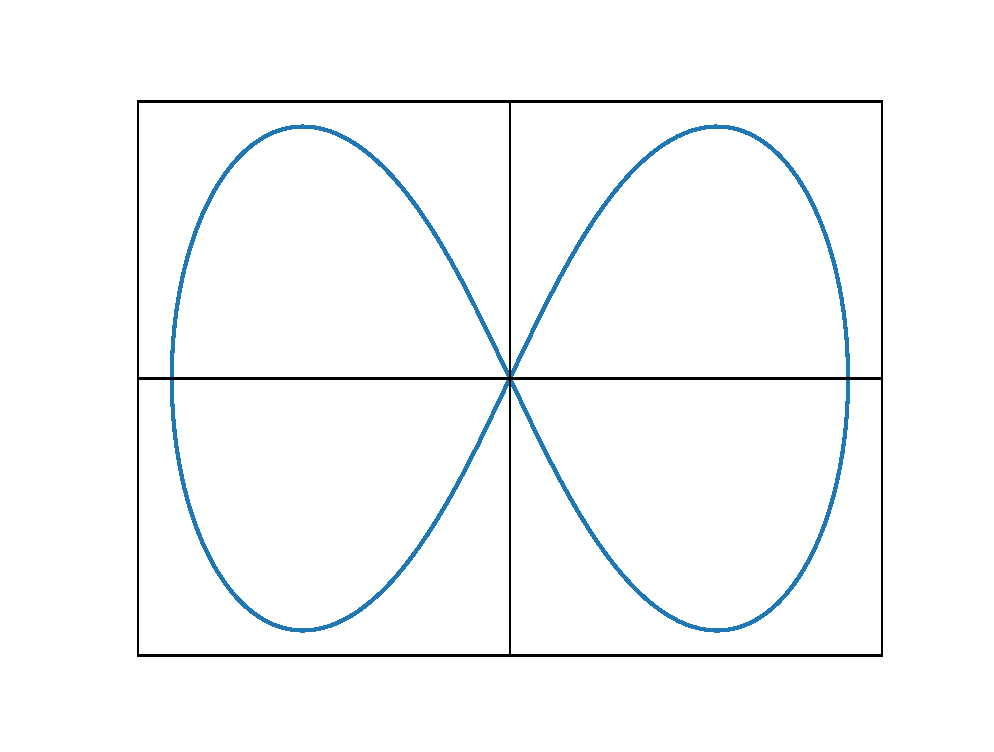
\includegraphics[scale=0.54]{Imagenes/plot_leminscata_01.eps}
    \caption{Gráfica de la lemniscata.}
    \label{fig:figura_lemniscata}
\end{wrapfigure}
La curva se parece a un ocho invertido, teniendo al eje x como eje de simetría, pasa en dos ocasiones por el origen, como se puede ver en la figura (\ref{fig:figura_lemniscata})
\par
Para esta curva, por simetría se tiene la misma longitud en cada uno de los cuatro cuadrantes, por lo que podemos calcular la longitud en el primer cuadrante y luego multiplicarla por cuatro.
\par
Los puntos donde la curva cruza el eje $x$ en el origen son aquellos para los cuales el argumento del coseno es un múltiplo entero, impar de $\pi / 2$.  Para el tramo en el primer cuadrante, tomamos $0 \leq \theta \leq \pi/4$.
\par
La longitud de la curva en coordenadas polares es
\begin{align*}
s = \int_{\alpha}^{\beta} \left[ \rho^{2} + \left( \dv{\rho}{\theta} \right)^{2} \right]^{1/2} \dd{\theta}
\end{align*}
Como $\rho^{2} = a^{2} \, \cos 2 \theta$, tenemos que:
\begin{align*}
\left( \dv{\rho}{\theta} \right)^{2} = \dfrac{a^{4} \, \sin^{2} 2 \theta}{a^{2} \, \cos 2 \theta}
\end{align*}
Entonces:
\begin{align*}
\dfrac{1}{4} \, s &= \int_{0}^{\pi/4} \left( a^{2} \, \cos 2 \theta + \dfrac{a^{4} \, \sin^{2} 2 \theta}{\cos 2 \theta} \right)^{1/2} \dd{\theta} = \\[1em]
&= \int_{0}^{\pi/4} a \, \cos^{-1/2} 2 \theta \dd{\theta}
\end{align*}
Haciendo un cambio de variable, es posible llevar esta integral a una forma de la función Beta con integral. Sea $2 \theta = t$, por lo que el intervalo de integración ahora va de $0$ a $\pi/2$.
\par
Por tanto:
\begin{align*}
\int_{}^{\pi/4} a \, \cos^{-1/2} \, 2 \, \theta \dd{\theta} = \dfrac{a}{2} \int_{0}^{\pi/2} \cos^{-1/2} \, t \, \sin^{0} t \dd{t}
\end{align*}
De uno de las identidades para expresar la función Beta:
\begin{align*}
B(x, y) = \int_{0}^{\pi/2} 2 \, \sin^{2x-1} \theta \, \cos^{2y-1} \theta \dd{\theta}
\end{align*}
tenemos que:
\begin{align*}
\dfrac{1}{4} \, s &= \int_{0}^{\pi/4} a \, \cos^{-1/2} 2 \theta \dd{\theta} =  \\[0.5em]
&= \dfrac{a}{2} \int_{0}^{\pi/2} \cos^{-1/2} t \, \sin^{0} t \dd{t}
\end{align*}
Encontramos entonces:
\begin{align*}
\dfrac{1}{4} \, s &= \dfrac{a}{2} \, \dfrac{1}{2} \, B \, \left(\dfrac{1}{4}, \dfrac{1}{2} \right) = \\[1em]
&= \dfrac{a}{4} B\left(\dfrac{1}{4}, \dfrac{1}{2} \right)
\end{align*}
La longitud completa de la lemniscata se obtiene al multiplicar el resultado anterior por cuatro, además ocupamos la fórmula que relaciona la función Beta con la función Gamma. Así tenemos el resultado:
\begin{align*}
s &= a \, B\left(\dfrac{1}{4}, \dfrac{1}{2} \right) = \dfrac{a \, \Gamma \left( \dfrac{1}{4} \right) \, \Gamma \left( \dfrac{1}{2} \right) }{\Gamma \left( \dfrac{3}{4} \right)} = \\
&= \dfrac{4 \, a \, \Gamma \left( \dfrac{5}{4} \right) \sqrt{\pi}}{\dfrac{4}{3} \, \Gamma \left( \dfrac{7}{4} \right)} \cong 5.2 \, a
\end{align*}

\subsection{Período de oscilación de un péndulo.}

Se nos pide calcular el período de oscilación de un péndulo simple que oscila en un arco de $\ang{180}$, como se aprecia en la figura (\ref{fig:figura_pendulo_simple}):
\begin{figure}[H]
    \centering
    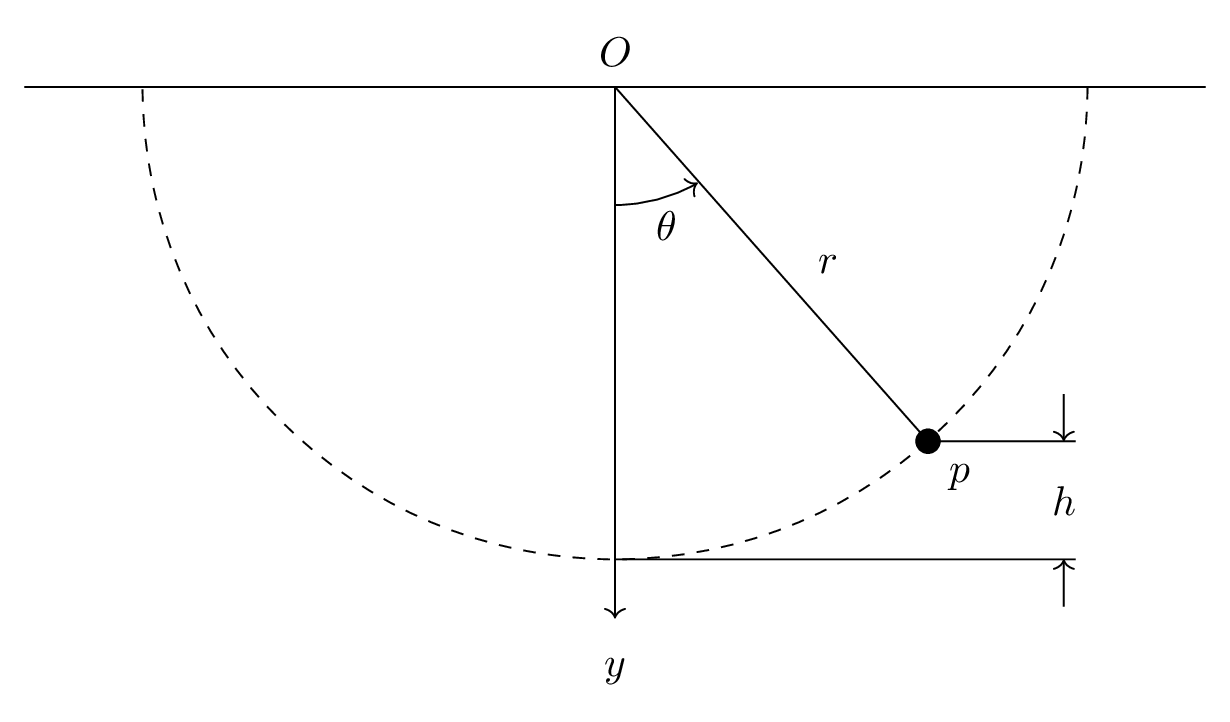
\includegraphics{Figuras/pendulo_simple}
    \caption{Esquema del péndulo simple que oscila en un arco.}
    \label{fig:figura_pendulo_simple}
\end{figure}
Usando el eje coordenado, vemos que el ángulo polar $\theta$ varía de $-\pi/2$ a $\pi/2$, mientras que la coordenada radial $r = Op$ permanece constante. Sea $g$ la aceleración debida a la gravedad y $W$ el peso del péndulo $p$.
\par
La energía potencial de $p$ en $\theta = 0$ es cero. Por lo que el valor de la energía potencial en cualquier instante, es el producto de $W$ por la altura $h$:
\begin{align*}
P = W (r - r \, \cos \theta)
\end{align*}
Mientras que la energía cinética viene dada por
\begin{align*}
K = \dfrac{m \, v^{2}}{2} = \dfrac{1}{2} \, \dfrac{W}{g} \left( r \, \dv{\theta}{t} \right)^{2}
\end{align*}
Como el péndulo está oscilando, la energía total es constante: $P + K = C$. Lo que nos permite expresar una ecuación diferencial del movimiento:
\begin{align*}
W \, r (1 - \cos \theta) + \dfrac{1}{2} \dfrac{W}{g} \left( r \dv{\theta}{t} \right)^{2} = C
\end{align*}
Para calcular $C$ tomamos el tiempo $t = 0$ cuando $\theta = \pi/2$, vemos que el péndulo está en reposo, por lo que $\dv*{\theta}{t} = 0$, cuando $t = 0$ y $\theta = \pi/2$.
\par
De esta manera $C = W \, r$ y la ecuación de movimiento resulta
\begin{align*}
\dfrac{r}{2 \, g} \left( \dv{\theta}{t} \right)^{2} - \cos \theta = 0
\end{align*}
Como $p$ está oscilando de un lado a otro, $\dv*{\theta}{t}$ es en ocasiones positiva y en otras negativa; podemos estimar el período $T$, calculando el tiempo que tarda de ir de $\theta=0$ a $\theta=\pi/2$, para luego multiplicar el resultado por $4$.
\par
De esta manera podemos usar la raíz positiva para resolver la ecuación de $\dv*{\theta}{t}$. Entonces tenemos:
\begingroup
\allowdisplaybreaks
\begin{align*}
\sqrt{\dfrac{r}{2 \, g}} \, \dv{\theta}{t} &= \cos^{1/2} \theta \dd{t} = \\[1em]
\dd{t} &= \sqrt{\dfrac{r}{2 \, g}} \, \dv{\theta}{t} \cos^{-1/2} \theta \dd{\theta} = \\[1em]
T &= 4 \, \sqrt{\dfrac{r}{2 \, g}} \, \int_{0}^{\pi/2} \cos^{-1/2} \theta \dd{\theta} = \\[1em]
&= 2 \, \sqrt{\dfrac{r}{2 \, g}} \, \int_{0}^{\pi/2} 2 \, \sin^{0} \theta \, \cos^{-1/2} \theta \dd{\theta} = \\[0.8em]
&= \sqrt{\dfrac{2 \, r}{g}} \, B \left( \dfrac{1}{2}, \dfrac{1}{4} \right) = \\[0.8em]
&= \sqrt{\dfrac{2 \, r}{g}} \, \dfrac{\Gamma \left(\dfrac{1}{2} \right) \, \Gamma \left(\dfrac{1}{4} \right)}{\Gamma \left(\dfrac{3}{4} \right)} = 
\end{align*}
\endgroup
\begin{align*}
T = \sqrt{\dfrac{2 \, r}{g}} \, \dfrac{\Gamma \left(\dfrac{1}{2} \right) \, 4 \, \Gamma \left(\dfrac{5}{4} \right)}{\dfrac{4}{3} \, \Gamma \left(\dfrac{7}{4} \right)}
\end{align*}
Lo que nos falta es un paso: calcular los valores de la función Gamma. Usando los valores para la función Gamma, se concluye que
\begin{align*}
T \cong 7.416 \sqrt{\dfrac{r}{g}}
\end{align*}
Considera que se han omitido pasos en el desarrollo, pero en tus ejercicios deberán de estar lo más completo y detallados posible.

\section{Ejercicios a cuenta.}

Para que puedas repasar lo revisado para las funciones Gamma y Beta, se presentan dos ejercicios. Recuerda que debe de haber una demostración de la fórmula o expresión que ocupes tanto para la función Gamma y/o Beta que requieras.

\begin{enumerate}
\item  Demuestra que:
\begin{align*}
\Gamma \left( \dfrac{1}{2} - n \right) \, \Gamma \left( \dfrac{1}{2} + n \right) = (-1)^{n} \, \pi
\end{align*}
\item En una distribución tipo Maxwell la fracción de partículas moviéndose con velocidad $v$ y $v +\dd{v}$ es
\begin{align*}
\dfrac{\dd{N}}{N} = 4 \, \pi \left( \dfrac{m}{2 \, \pi \, k \, T} \right)^{3/2} \: \exp \left( - \dfrac{m \, v^{2}}{2 \, k \, T} \right) \: v^{2} \dd{v}
\end{align*}
donde $N$ es el número total de partículas. 
\par
El promedio o valor esperado de $v^{n}$ se define como $\displaystyle \expval{v^{n}} = N^{-1} \int v^{n} \dd{N}$.
\par
Demostrar que:
\begin{align*}
\expval{v^{n}} = \left( \dfrac{2 \, k \, T}{m} \right)^{n/2} \dfrac{\left( \dfrac{n + 1}{2} \right) !} { \left( \dfrac{1}{2} \right) !}
\end{align*}
\item Se muestra en la figura (\ref{fig:figura_cicloide}) parte de una cicloide cuyas ecuaciones paramétricas son
\begin{align*}
x &= a (\theta + \sin \theta) \\[0.5em]
y &= a (1 - \cos \theta)
\end{align*}
\begin{figure}[H]
    \centering
    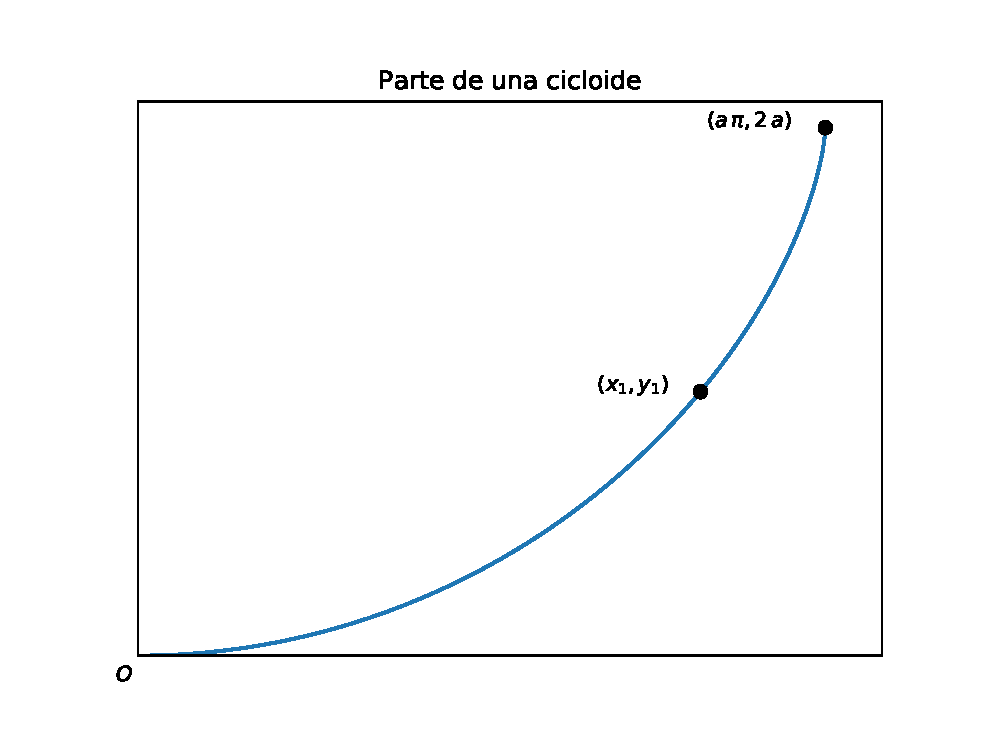
\includegraphics[width=0.75\textwidth]{Imagenes/plot_cicloide.eps}
    \caption{Una partícula deslizándose sobre una cicloide.}
    \label{fig:figura_cicloide}
\end{figure}

Demuestra que el tiempo que tarda una partícula para deslizarse sin fricción a lo largo de la curva desde el punto $(x_{1}, y_{1})$ hasta el origen, está dado por
\begin{align*}
t = \sqrt{\dfrac{a}{g}} \, \int_{0}^{y_{1}} \dfrac{\dd{y}}{\sqrt{y \, (y_{1}- y)}}
\end{align*}
Sugerencia: Demuestra que la longitud del elemento de arco es
\begin{align*}
\dd{s} = \sqrt{\dfrac{2 \, a}{y}} \dd{y}
\end{align*}
Evalúa la integral para demostrar que el tiempo es independiente de la posición inicial $y_{1}$.
\end{enumerate}
\end{document}